%1747
\newpage
\subsection{例題4-8 オリジナルの面を作ってみよう}


\begin{description}
    \item \textgt{\bf  考え方}
\end{description}

ジャンプアップゲーム(jump.hsp)のプログラムを改造してゲームで使われている\ruby{面}{めん}(マップ)を変えてみましょう。

プログラムを編集することで、面のデータを自分で変えることができます。

以下の場所を探して修正します。


\begin{figure}[H]
    \begin{center}
      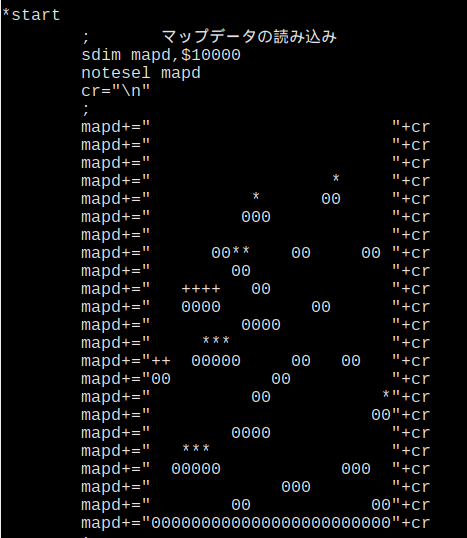
\includegraphics[keepaspectratio,width=10.478cm,height=12.07cm]{text04-img/s_jumpmapsrc.png}
    \end{center}
    \label{fig:prog_menu}
\end{figure}



\begin{description}
    \item \textgt{\bf \ \ 「0」はレンガ(壁)になります。}
    \item \textgt{\bf \ \ 「*」はコイン、「+」は矢になります。}
    \item \textgt{\bf \ \ マップデータが書かれている場所を探して、自分だけの面を作ってみましょう。}
\end{description}

でたらめに書き直してもエラーが出るだけです。必ず、

\begin{description}
    \item \textgt{\bf \ \ mapd+=” \ \ \ \ \ \ \ \ \ \ \ \ \ \ \ \ \ \ \ \ \ \ \ \ \ \ \ \ “+cr}
\end{description}

という形になるようにしてください。

文字は「”」で囲み、最後に「+cr」を入れます。

面のデータは、縦・横方向に広げることができます。


\begin{description}
    \item \textgt{\bf 例題4-8 答え}
\end{description}

ゲームを改造することで、難しくなったり、簡単になったりします。

改造ができたらTAや周りの友達にも見せてあげましょう。

%1820